\subsection{Ocean validation and far-cloud controls}
\label{sec:result-ocean_far_cldl}

Present ATom, shipborne EM27/SUN, and the far-cloud/clear-day cases where the
correction is nearly inert. Treat these as independent corroboration, not as
equivalent in statistical weight to TCCON. State the limited sample and
reference-scale caveats.


After we validate the correction of the \emph{DE} model in Sect.~\ref{sec:result-tccon_val,sec:result-corr_smooth}, we extend our validation to two different in-situ measurements to provide more validation tests over the ocean, considering that all TCCON stations are still over land and only part of them are close to the ocean coastline. We identify 17 ATom and OCO-2 co-located legs and 4 shipborne (MORE-2 and MR21-01) and OCO-2 co-located legs. We construct the pseudo-column \xcoatom from the in-situ airborne \xco measurement for comparison (Sect.~\ref{sec:method-eval-obs-xco2}), and use \xcoship directly as no prior profiles and averaging kernels are available.


Across the 17 ATom legs (14 near-cloud), the near-cloud improvement is a scatter reduction, not an offset shift. The median $|$residual$|$ ($|$\xcooco - \xcoatom$|$) falls from 0.53 to 0.45 ppm and the across-leg spread from ±0.72 to ±0.58 ppm, while the signed mean bias is essentially unchanged (+0.19 → +0.20 ppm, well within the per-leg pseudo-column $\sigma$ of 0.10–0.19 ppm). The far-cloud date (9 October 2017) is a negative control that the correction leaves nearly unchanged (Fig.~\ref{fig:ocean-validation}a, b). Against the shipborne EM27/SUN spectrometers (4 cases, 3 near-cloud), the correction collapses footprint scatter (mean $\sigma$ 0.63 → 0.27 ppm, against a mean ship reference $\sigma$ of 0.29 ppm) without moving the clear-sky control day (22 June 2019). The increase of $|$residual$|$ ($|$\xcooco - \xcoship$|$) absolute offset (all-case mean +0.99 ± 0.70 before, +1.18 ± 0.81 ppm after) could be dominated by reference-scale differences, considering no prior profiles and averaging kernel-harmonization applied  (Fig.~\ref{fig:ocean-validation}c, d). Note that we have limited temporal and spatial overpass samples compared to TCCON validations for ATom and Shipborne measurements comparison. The comparison with ATom in-situ and shipborne EM27/SUN measurements should be treated as independent corroboration, not as equivalent in statistical weight to TCCON.


Figure~\ref{app-fig:atom_far_cld,app-fig:ship_far_cld} illustrate little change in values and distribution for far-cloud footprints for ATom and Ship observation cases. These two negative controls are consistent with the far-cloud behavior in the TCCON comparison itself. In the station-day groups beyond the
production reference radii (ocean $\geq 5$~km, land $\geq 15$~km; Table~\ref{tab:model_comparison}), the pre-correction error is already small, and the correction leaves it slightly improved rather than degraded (footprint RMSE 1.02 $\rightarrow$ 0.86 and 0.95 $\rightarrow$ 0.79~ppm, respectively; see also the cloud-distance dependence in Fig.~\ref{app-fig:qf01_DE_eval}), so the near-inert far-cloud response over the ocean is not a small-sample artifact.



\begin{figure}[t]
\centering
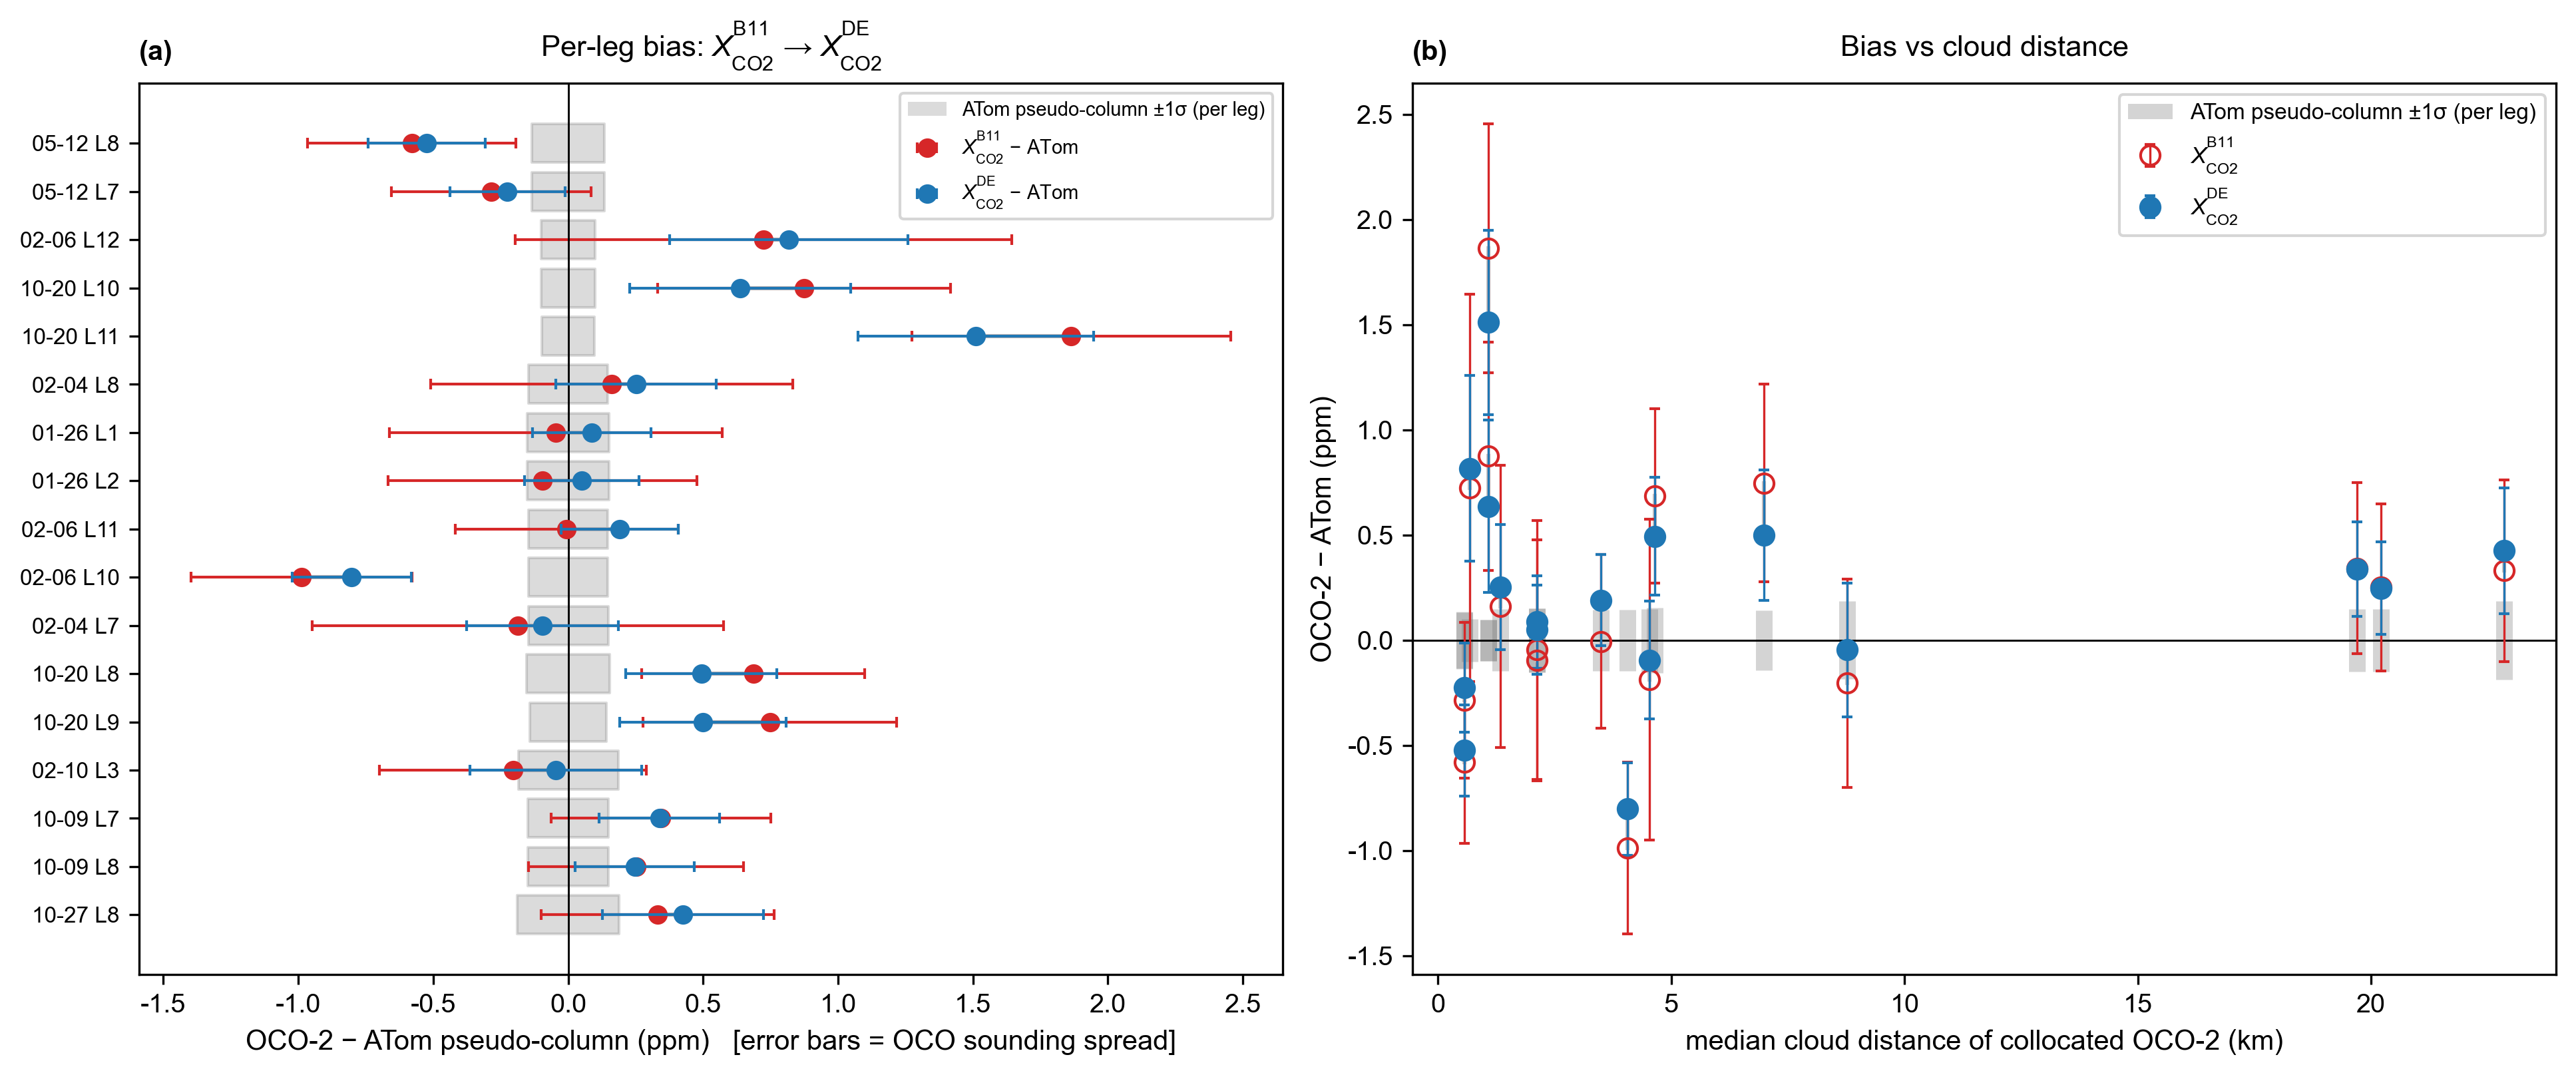
\includegraphics[width=0.95\textwidth]{figures/fig11a_atom_summary.png}\\[4pt]
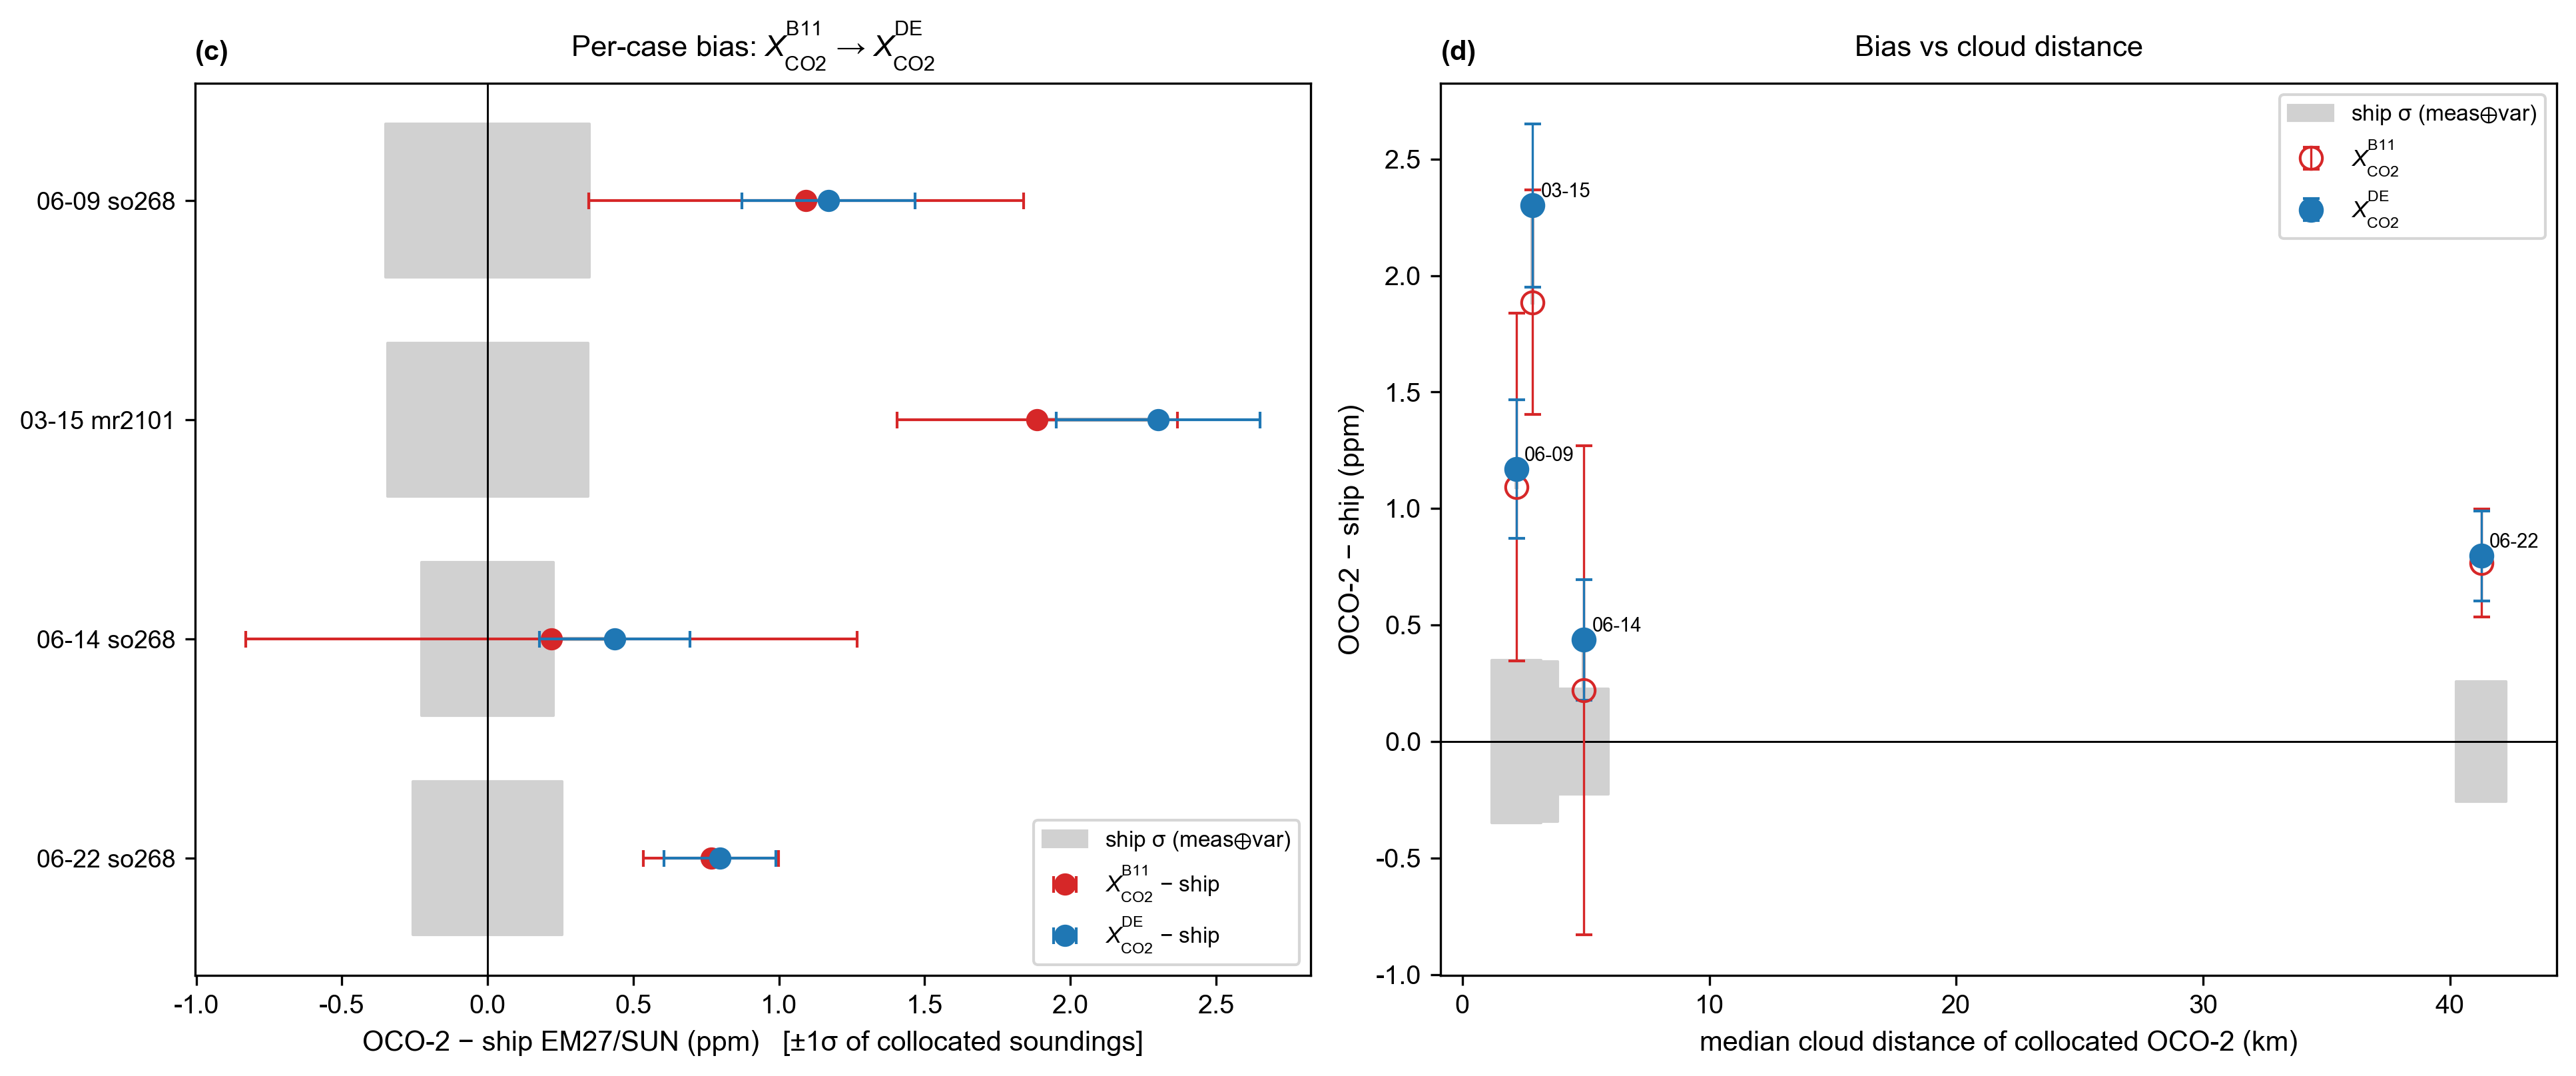
\includegraphics[width=0.95\textwidth]{figures/fig11b_ship_summary.png}
\caption{Independent ocean corroboration. (a, b) ATom aircraft pseudo-column comparison (8 dates, 17 collocated legs, AK-smoothed; the unmeasured stratosphere is filled with the OCO-2 prior so it cancels in the comparison), including the far-cloud negative-control date (9 October 2017): per-leg signed bias before and after correction, and the same residuals against median cloud distance; grey bands mark each leg's own pseudo-column ±1σ. (c, d) Shipborne EM27/SUN comparison (R/V Sonne MORE-2 and R/V Mirai MR21-01; 100 km / ±2 h), including the clear-sky control day (22 June 2019), in the same two views; grey bands mark the ship reference uncertainty (measurement ⊕ within-window variability).}
\label{fig:ocean-validation}
\end{figure}





\FloatBarrier